\documentclass{jot}

\usepackage[english]{babel}
\usepackage{microtype} % optional, for aesthetics
\usepackage{tabularx} % nice to have
\usepackage{booktabs} % necessary for style
\usepackage{mathtools}
% \usepackage{graphicx}
% \graphicspath{{./figures/}}
% \usepackage{listings}
% \lstset{...}

% \newcommand\code[1]{\texttt{#1}}
% \let\file\code

\graphicspath{{images/}}


%%% Article metadata
\title{Main project: Song Recommendation System}
\runningtitle{Main project: Song Recommendation System}

\author[affiliation=UiT, nowrap]
    {Madhu Koirala}
    {is a master student in Computer Science at the University of Troms\o. You can contact him at \email{mko075@uit.no}.}

\author[affiliation=UiT, nowrap]
    {\'{A}lvaro Mart\'{i}nez Fern\'{a}ndez}
    { is a master student in Computer Science at the University of Troms\o. You can contact him at \email{afe026@uit.no}.}

\affiliation{UiT}{University of Troms\o, Norway\\
\url{https://uit.no/startsida}}

\runningauthor{Madhu Koirala and \'{A}lvaro Mart\'{i}nez}

\jotdetails{
    year=2020,
}


\begin{document}

\begin{abstract}
Looking for the information that we are interested in can be a tedious process nowadays because of the large amounts of data that we need to navigate. Looking for media content such as songs or movies can be even harder, since it’s difficult to know if we will like the content. Recommendation systems can help users in the decision process by filtering the content based on the content that the user likes and consumes most. In this project we implement a song recommendation system using collaborative filtering approach. The model that we use consists of several users and each user has a list of songs that the user usually listens to. By using collaborative filtering, song recommendations are done by recommending songs from users with similar taste using Jaccard similarity. Also, a simple approach which uses popularity of songs (number of users and listen counts) has been implemented. Both methods show a list of recommended songs for a user and a comparison between them with the help of precision recall curve proves a better performance of similarity-based approach.
\end{abstract}

\keywords{Recommendation systems, recommendation methods, music recommendations, machine learning}

\tableofcontents

\section{Introduction}
One of the main problems nowadays when using the internet is the overwhelming amount of data that we get and that we need to filter. Looking for the information that we want can be a tedious and boring task. There are some tools like search engines that help the user filter the content, some examples are Google\footnote{https://google.com} or Yahoo\footnote{https://www.yahoo.com}. Modern systems include new recommendation algorithms that automatically filter the content for the user, based on the information that the user has consumed. This is very common in multimedia platforms like Netflix\footnote{https://www.netflix.com} or Spotify\footnote{https://www.spotify.com}. Lists of recommended media are shown to the user with content that it may be of interest, based on the user’s interests. This is very helpful since looking, for instance, for songs that we may like can be very hard and we need to use a lot of time. Also when looking for a film that we are interested in on Netflix can be a cumbersome process. Thanks to recommendation algorithms, this content can be automatically filtered.

There are different ways to build a recommendation system. Some approaches are by using information based on the user’s preferences, item features, factors such as time, season, etc. In the literature we can find four methods to implement a recommendation algorithm: content based, collaborative filtering, knowledge-based method and hybrid method. We will explain now each of these methods in more detail.

\subsection{Content Based Method}
This method depends on the attributes of objects or items and user profile to make recommendations to its users. For instance, in a movie recommendation system, the name of the movie is an item or object and so is the name of actors, the year it was produced and the genre or genres of the movie such as romance, action, comedy, etc. Focus on Table \ref{tab:content-based} to understand how exactly this method works.\\
\begin{table}[h!]
\begin{tabular}{lllll}
Movie                & User 1 & User 2 & Attribute 1(romance) & Attribute 2(Action) \\
Love for Seven Lives & 4      & 5      & 0.9                   & 0.1                  \\
Against Injustice    & 5      &        & 0.1                   & 0.8                  \\
You n Me             & 4      &        & 0.7                   & 0.2                  \\
Earn Kr 1 Spend 10   &        & 1      & 0.1                   & 0.4                  \\
\end{tabular}
\caption{Content based example}
\label{tab:content-based}
\end{table}

If we are to decide if User 2 likes the movie You n Me, we need to consider her profile and the attributes of the movie. She likes Love for Seven Lives, which has high romance and almost no action. Based on this, she has a certain profile. When we match this profile and the attributes of You n Me, it’s highly likely that she will love this movie. So, we recommend this movie to her.

Content-based recommender system has the advantage that it does not require information about other users. It only needs to know what the current user is interested in. Also, it can recommend niche products as it analyses the interests of a user only and niche items are the goods specific for a particular customer base. However, there are some disadvantages too. We need to create the entire domain of sufficient knowledge of the items, such as genre, texts to explain the item, and other information which can be used to select the item of recommendation. Another demerit is it only makes recommendations around the interest of a user that it knows. If the user also likes some other types of items, it does not know because the user has never bought it.


\subsection{Collaborative Filtering}
This technique is entirely based on users' interaction with the items. Based on the ratings they have provided, it calculates similarity between the users. If a similarity is found, for example between A and B users, then, the system recommends the items liked by A to B.
Let’s try to make it clear with the help  of an example of a music recommendation system. In Table \ref{tab:collaborative-filtering} we present information about music ratings for four users.\\

\begin{table}[h!]
\centering
\begin{tabular}{lllll}
Users & Music A & Music B & Music C & Music D \\
M     & 5       & 2       &         &         \\
N     & 2       &         & 5       & 5       \\
O     & 3       & 3       & 3       &         \\
P     & 1       & 3       &         &         \\
\end{tabular}
\caption{Collaborative filtering example}
\label{tab:collaborative-filtering}
\end{table}

The system tries to calculate the similarities between the users based on the ratings given by them. Similarity is found using the formula of Cosine Similarity.

\[Sim(M,N) = \cos (\theta) = \frac{M.N}{|M|.|N|}\]

If we try to find similarity between the users M and N, we need to take the values which are rated by both the users. Music A has been rated by both of them.
\[\cos(\theta) = \frac{2.5}{\sqrt{2^2+2^2} * \sqrt{2^2 + 5^2 + 5^2}}) = 0.252\]

The value of cos varies between 0 and 1. When the angle is 90 degrees, the two vectors are orthogonal which indicates there is no similarity at all and a zero degree between the vectors show they are exactly the same. In the above example, the similarity value is 0.252, which is not good enough for recommendation.
One good aspect of this system is it does not require any domain knowledge as it can recommend an item based on the similarity of users according to their feedback. The other advantage is it may be able to recommend all types of items unlike content-based which always advise similar items. For instance, users A and B and C love folk music. And B and C also like pop music. Looking at the similarity between these users, it might be good to recommend pop music to user A. On the other hand, this system can suffer from ‘cold start’ problem. If we already have a number of interactions between various users and items then only it can recommend an item. But initially it does not have any information about users’ likings to give suggestions. So, for a fresh item or user who does not have much interaction data, it does not make a good recommendation. Also, it suffers from the problem of sparsity. In a real-world situation where there are millions of items and users, no matter how much interaction has been made but still there can be items and users with very few interactions. This can lead to ‘not good ’ recommendations. Last disadvantage it can have is scalability. It will require huge computation in a practical scenario where there is a huge dataset of users and items.


\subsection{Knowledge-Based Method}
This system collects users’ preferences, interests, their profile such as age, place and makes recommendations. Based on the input provided by the users, it finds similarity between their profiles and can advise the items.
It does not require any interaction data and the recommendations can be quite good because the users have themselves set their interests and likes. On the down side, we need users to fill in their data and at times we may have to be careful about privacy concerns also.


\subsection{Hybrid Method}
This method combines all three techniques content-based, collaborative filtering and knowledge-based so that the individual drawbacks are cancelled out.

\section{Background and Related Work (state of the art)}
A music recommendation system is a specialized information retrieval system for multimedia content\cite{chung_kim_2018}. A recommendation system\cite{isinkaye_folajimi_ojokoh_2015} is defined as a system that searches through a large volume of information in order to filter the information based on the personalized preferences of the user. It is also seen as a decision making strategy for users under complex information environments. Originally recommender systems were defined as a way to assist the social process of using recommendations of others in order to make choices when there is not sufficient personal knowledge of the different alternatives\cite{resnick_varian_1997}.

There are several approaches in the literature for the implementation of recommendation systems: content-based, collaborative filtering, knowledge-based and hybrid method. Machine learning and deep learning techniques have been used to enhance recommendation algorithms. In a study about recommendation systems\cite{singhal_sinha_pant_2017}, an analysis of the literature shows that machine learning and deep learning has been used especially for collaborative filtering algorithms.

We can think of many ways to extract properties or features from the objects that we want to recommend. As for this project we will extract information from the songs such as genre, artist, title or album. In other works other properties are taken into account like in this study\cite{park_yoo_cho_2006}, where they build a music recommendation system based on the context or environment of the listener such as day, time, temperature, if it is rainy, cloudy or sunny, etc. In another study\cite{ayata_yaslan_kamasak_2018} they even measure the mood of the user by using a galvanic skin response and photoplethysmography.

When analyzing related work about recommendation systems, we can find many studies that use the different methods mentioned before. We can see that content-based systems are mostly used when we are not using or cannot use metadata. For instance in this study\cite{cano_koppenberger_wack_2005} they build a music recommendation system that extracts descriptions related to instrumentation, rhythm and harmony from music audio signals. However in our project we are using metadata since we use a collaborative filtering approach, in this case music that the user likes by tagging the songs as favorites. In some recommendation systems\cite{choi_yoo_kim_suh_2012}\cite{debnath_ganguly_mitra_2008}, both collaborative and content based approaches are used, resulting in a hybrid approach. In this way the advantages from each method are used in order to enhance the accuracy of the recommendation system.

\section{Problem to be solved and Aims}
The goal of our project is to design a music recommendation system. There are many methods of implementing a recommender system. We have used a collaborative filtering algorithm as it is the most used approach in the real world.
The problems that we had anticipated to face to accomplish our goal are as below: We will discuss these issues in the discussion part.
\begin{enumerate}
  \item How to implement collaborative filtering approach in a music recommender system?
  \item Which particular algorithm will give the optimum performance in our case?
  \item What kind of dataset do we require for training and validation of our model and how can we find the right one?
  \item Which machine learning algorithm do we need to use for the best results?
  \item How do we train and validate our model?
\end{enumerate}

\section{Contribution}
A recommendation system for songs can be very practical in many applications and services nowadays. With the Internet, people can easily have access to endless multimedia content like music. Also the potential that there is at the moment to find new music and get good recommendations is enormous thanks to machine learning and recommendation systems. We present here an example of how to implement a song recommendation system using a collaborative filtering algorithm.

We have implemented the song recommendation system using Python and some packages like sklearn and pandas used for machine learning. We have also built a small graphic user interface that shows potential recommendation songs for a user.

As for the evaluation we have compared the collaborative filtering solution with a more primitive one, a popularity based algorithm. We couldn’t evaluate how good the recommended songs were, since this can be a bit subjective to each user.

\subsection{Architecture and design}
The song recommendation system is built using a machine learning technique. The dataset used in the system contains information about users, songs that the users have listened to and how many times they have listened to a particular songs. This dataset comes from the Million Song Dataset\cite{millionsongs} and in particular we use two files from this dataset. The first dataset\footnote{https:\/\/static.turi.com\/datasets\/millionsong\/song\_data.csv} is the metadata file which contains song ID and related information about the songs. The second one\footnote{https:\/\/static.turi.com\/datasets\/millionsong\/10000.txt} is the rating dataset containing the user ID, song ID and the number of times the songs have been heard by the users. In the system we train the dataset and make 2 types of recommendations, one that is popularity based and a second one that is personalized for each user. In Figure \ref{fig:architecture} we can see an overview of the architecture of the system.

\begin{figure}[h!]
    \centering%
    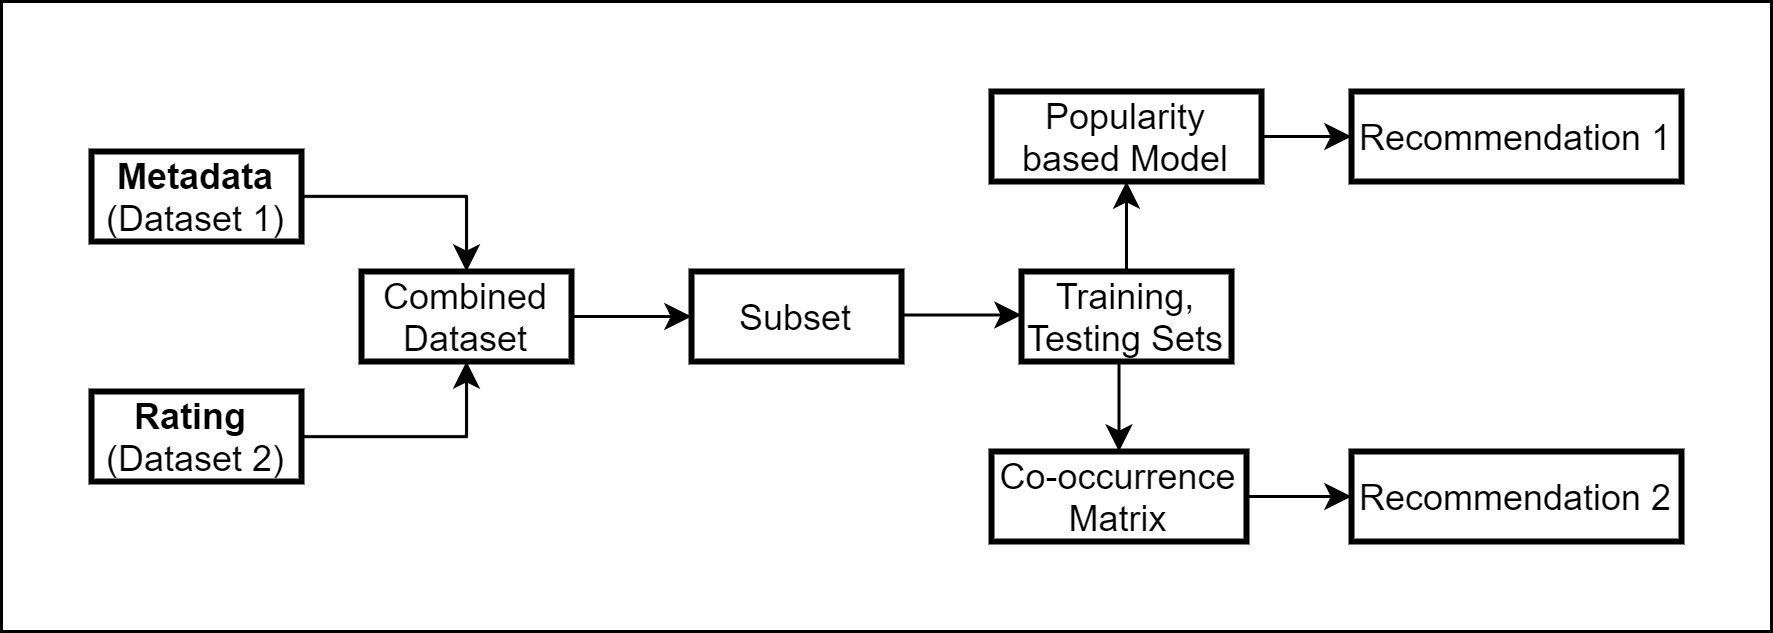
\includegraphics[width=\textwidth]{architecture}
    \caption{Architecture of the system.}
    \label{fig:architecture}
\end{figure}%

The initial step that we do is to combine the two datasets and then remove duplicates that this merging causes and ending up with a new dataset that contains the following fields: User ID, Song ID, Listen Count, Song Title, Release, Artist Name and Release Year. Then a subset of 15000 entries from the dataset is taken since the original dataset is too large and for the purpose of this project it is enough with a smaller dataset. The subset is further split into two sets: training and testing sets, the former comprising 80\% of the dataset.

For recommendation, two strategies have been adopted. The first one is based on the popularity of songs which is directly related to the number of songs that have been listened to. And the second uses co-occurrence matrix which is a measure that calculates by what factor the items are related to each other. The algorithm used is Jaccard Similarity to find similarity between the items.

The popularity based model generates the same results irrespective of the user because it simply lists out the most popular songs. On the other hand, the co-occurrence matrix generates a personalized list of recommended songs for a specific user.\\

As for the design of the system we have used Python to develop the song recommendation system. For the machine learning logic we used pandas and sklearn Python packages. pandas is a data analysis and manipulation tool that helped us shape the dataset. sklearn was used to train the dataset using the function train\_test\_split, which split arrays or matrices into random train and test subsets.

We also built a small graphic user interface using the tkinter Python package, which is used for graphic interfaces. In the GUI we can see the song recommendation for a particular user, using the co-occurrence matrix approach. See Figure \ref{fig:design} for an example of the GUI.

\begin{figure}[h!]
    \centering%
    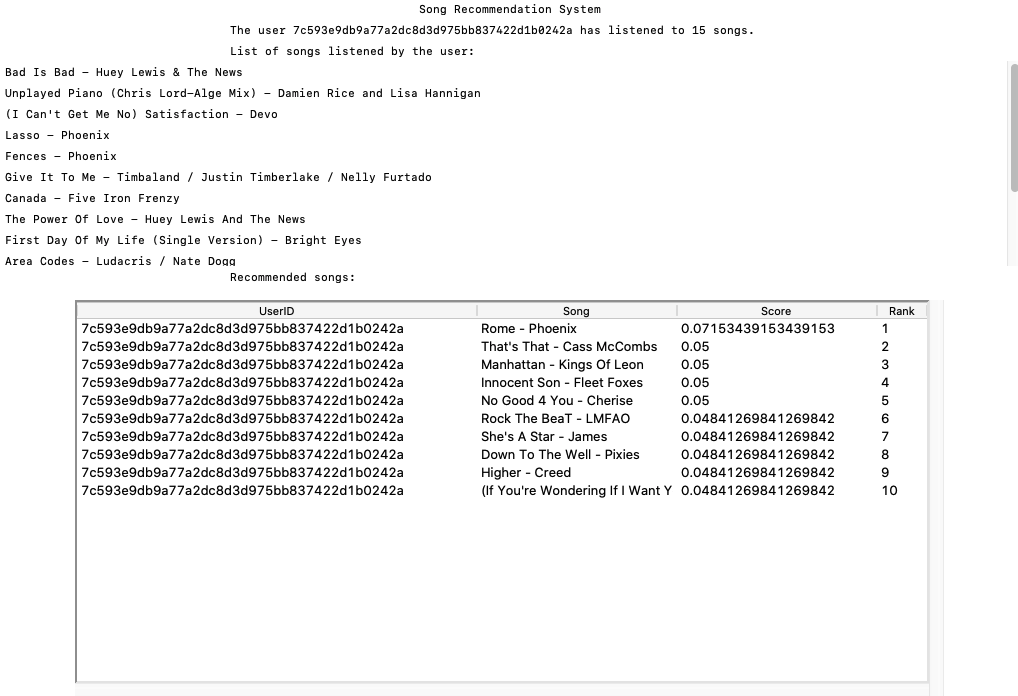
\includegraphics[width=\textwidth]{design}
    \caption{GUI for song recommendation for a particular user using the co-occurrence matrix approach.}
    \label{fig:design}
\end{figure}%

\subsection{Results and evaluation}
The program is able to produce recommendations for both popularity-based and similarity based approaches. Both of them provide top 10 recommendations. The first one produces same results as it just shows the most popular songs without giving any concern to the user, while the second one displays personalized  list of songs.
Figure \ref{fig:evaluation}. shows a precision recall curve, which will be used to interpret the results produced by these approaches. In this case, for our problem domain, what is important is the length that a song is listened to, that a number of users have all liked the song. Recall is in this case the “measure of the proportion of all relevant results included in the top results”. Precision is the measure  of the relevancy of songs in relation to the top ten results of a recommended song, whereas recall seeks to measure the relevancy of songs in relation to all the songs.
\\

\begin{figure}[h!]
    \centering%
    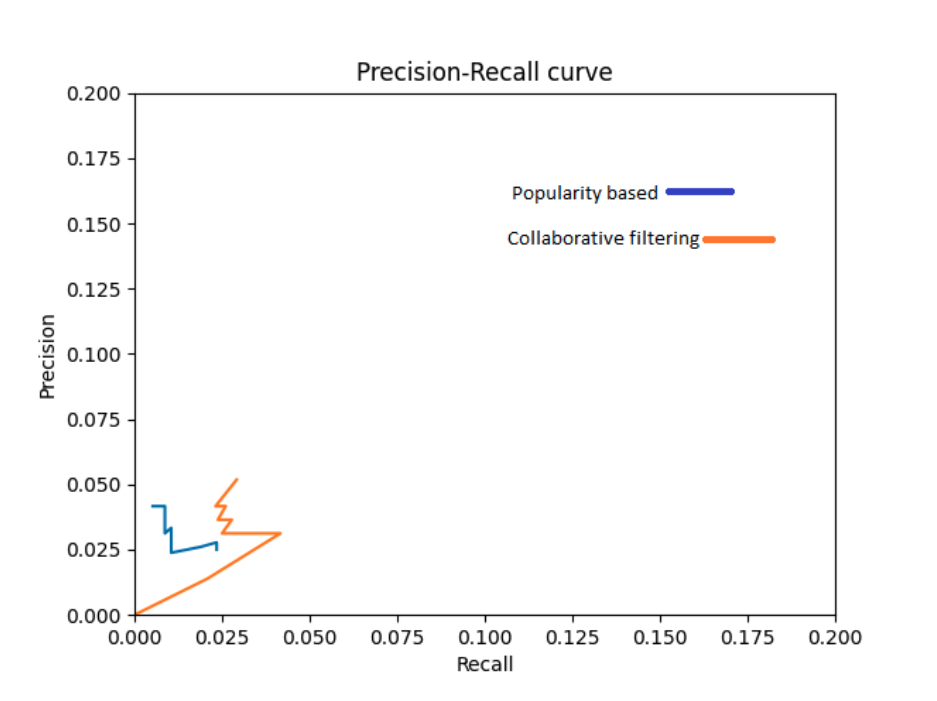
\includegraphics[width=0.9\textwidth]{evaluation}
    \caption{Precision-Recall curve.}
    \label{fig:evaluation}
\end{figure}%

The results have been evaluated using a very simple technique. The unique user ID ranges from 0 to 3862. A number of tests have been run to cover the whole range of user ID and results produced successfully. This shows that the system can make recommendations in all situations. Further, a verification is carried out by looking at the list of dataset and counting the number of listens, which showed that the result of popularity-based should be correct.
Similarly, we tried to trace out how many times the result shown by item-similarity approach appears in the dataset for a simple verification of the results. If it recommends an item which has been rated by only a single user of a few users, then we could possibly imagine that it might be producing a wrong result. Such cases were not found, approving of the methods we used.

\section{Conclusions, Discussion and further work}

After building this recommender system, there are few things we can outline, which are crucial for a collaborative recommendation system. First of all, we need to have a dataset containing the ratings provided by the user. This is also called user-interaction data and it is a must for collaborative approach. This approach is based on similarity of users or items and similarity is actually a function of ratings given by the users. There are a number of ways to calculate similarity and so many ways to make predictions. So, in the real world we have to be aware of all these methods and be able to use the particular methods best suited for a certain environment or situation. In this project, however more than evaluating the efficiency of a particular approach, we focussed on producing the results.

Precision Recall curve in Figure \ref{fig:evaluation} can be helpful in analyzing the performance of popularity and similarity based approaches. From the graph, we can conclude that similarity based approach gives more accurate results than naive popularity based approach, as the curve for similarity based method shows it works for much higher values of precision and recall compared with the other method.

The system now shows popularity-based and similarity-based recommendations separately. As a further work, we can work to produce popularity-based recommendations for new users who do not have any interaction data. This combining these approaches we can make a better system suited for both new as well as old users.

\backmatter

\nocite{*}
\bibliographystyle{alphaurl}
\bibliography{main}

% \newpage
\abouttheauthors

\end{document}
